\chapter{Methodology}
The aim of SRON-GAN is to be trained on a relatively small sample size of complex physical models and still be able to converge. After which SRON-GAN should be able to retrieve all features listed in Table \ref{table:exogandatasetparameters}. Considering the complexity of GANs, it is essential to initially start with the concept of ExoGAN and increase complexity from there. This leads to a simple SRON-GAN model, which is trained on a sample from the ExoGAN dataset. After which the SRON-GAN model trained on complex physical models is created. Within this chapter the data collection methods are introduced. Exploratory Data Analysis (EDA) on the raw data is performed. The EDA gives an insight into the raw data and the ways it has to possibly be transformed. This is followed up by the data processing pipeline. This pipeline converts the atmospheric models into the ASPAs which are used for training and testing. Finally, SRON-GAN is introduced, together with the method used to evaluate the models. It is worth noting that High Performance Computing (HPC) from both SURFsara and The Hague University of Applied Sciences is thoroughly used for nearly every step in this work. The data generation with ARCiS took 6 days using 15 virtual machines (4 cores per machine) and resulted in 250 GB of data. The complete ExoGAN dataset, including the processed ASPAs, has a size of 90 GB. All data processing was done using 24 cores, to minimise the run-time to minutes instead of hours. Model training has been done with four NVIDIA Tesla M10 GPU's and five NVIDIA GeForce RTX 2080 Ti's.



%%%%%%%%%%%%%%%%%%%%%%%%%%%%%%%%%%%%%%%%%%%%%%%%%%%%%%%%%%%%%%%%%%%%%%%%%%%%%%%%%%
\section{Data Collecting}
To create a dataset consisting transmission spectra made by using complex physical models, ARCiS is used to compute $1.3\cdot 10^5$ cloudy hot-Jupiter transmission spectra. The planet formation parameters are randomly sampled, after which ARCiS computes the transmission spectrum and its corresponding features. Like stated in Chapter \ref{atm_retrieval} both the planet formation parameters and features will be retrieved by SRON-GAN, henceforth they are called features. A complete list of the features is found in Table \ref{table:exogandatasetparameters}. Due to a bug in ARCiS the final dataset got reduced to $4.27\cdot10^4$ forward models. 

For the simple physical model a random selection of $1.3 \cdot 10^5$ simulations is taken from the already existing ExoGAN dataset, as described in Chapter \ref{exogan}. For both the simple and complex-physical model their respective datasets are separated in a train and test set. Both datasets are randomly split into a train and test set. The train set size is 70\% of the original dataset, whereas the test set contains the remaining 30\%.





%%%%%%%%%%%%%%%%%%%%%%%%%%%%%%%%%%%%%%%%%%%%%%%%%%%%%%%%%%%%%%%%%%%%%%%%%%%%%%%%%%
\section{Exploratory Data Analysis} \label{eda}
EDA is performed on both training datasets to gain insight into the original data. An example spectrum from the complex physical dataset is shown in Figure \ref{fig:h2obins}. The original distributions of the features from the complex physical modes are found in Figure \ref{fig:distribution_original}. The logarithmically sampled parameters are transformed back to their logarithmic scale, resulting in the distributions of Figure \ref{fig:distribution}. This allows for a higher spread in information, which in return allows for the neural network to learn this distribution more easily. The global minimum and maximum values per feature are calculated and stored to later on be used for normalisation. These values are found in Table \ref{table:min_max_values__models_features}. Considering that lots of features inside the spectra are relatively small, each spectrum is binned up into 17 bins. The bins are chosen in such a way that they maximally amplify the $\mathrm{H_2O}$ signature within the spectra, exact bin ranges are found in Table \ref{table:spectrum_bins_ranges}. Each bin is normalised by using the local bin minimum and maximum values. These minimum and maximum values are later on normalised by using the global spectrum minimum and maximum values, which are 4.94$\cdot$10$^{-4}$ and 0.108 respectively. Note that the EDA is only performed on the training datasets. Calculating the minimum and maximum values from only the training set ensures that there is no data leakage from the test set.

\begin{figure} [!htb]
    \centering
    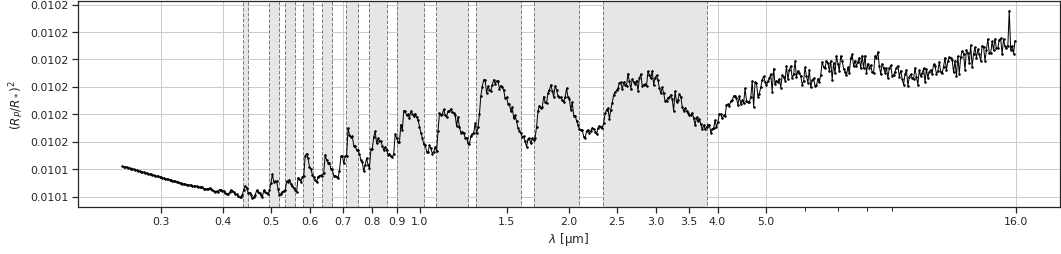
\includegraphics[scale=0.4]{figuren/H2O bins.png}
    \caption{A spectrum generated by ARCiS containing $\mathrm{H_2O}$. The grey bins highlight the H$_2$O signatures.}
    \label{fig:h2obins}
\end{figure}

\begin{figure} [!htb]
    \centering
    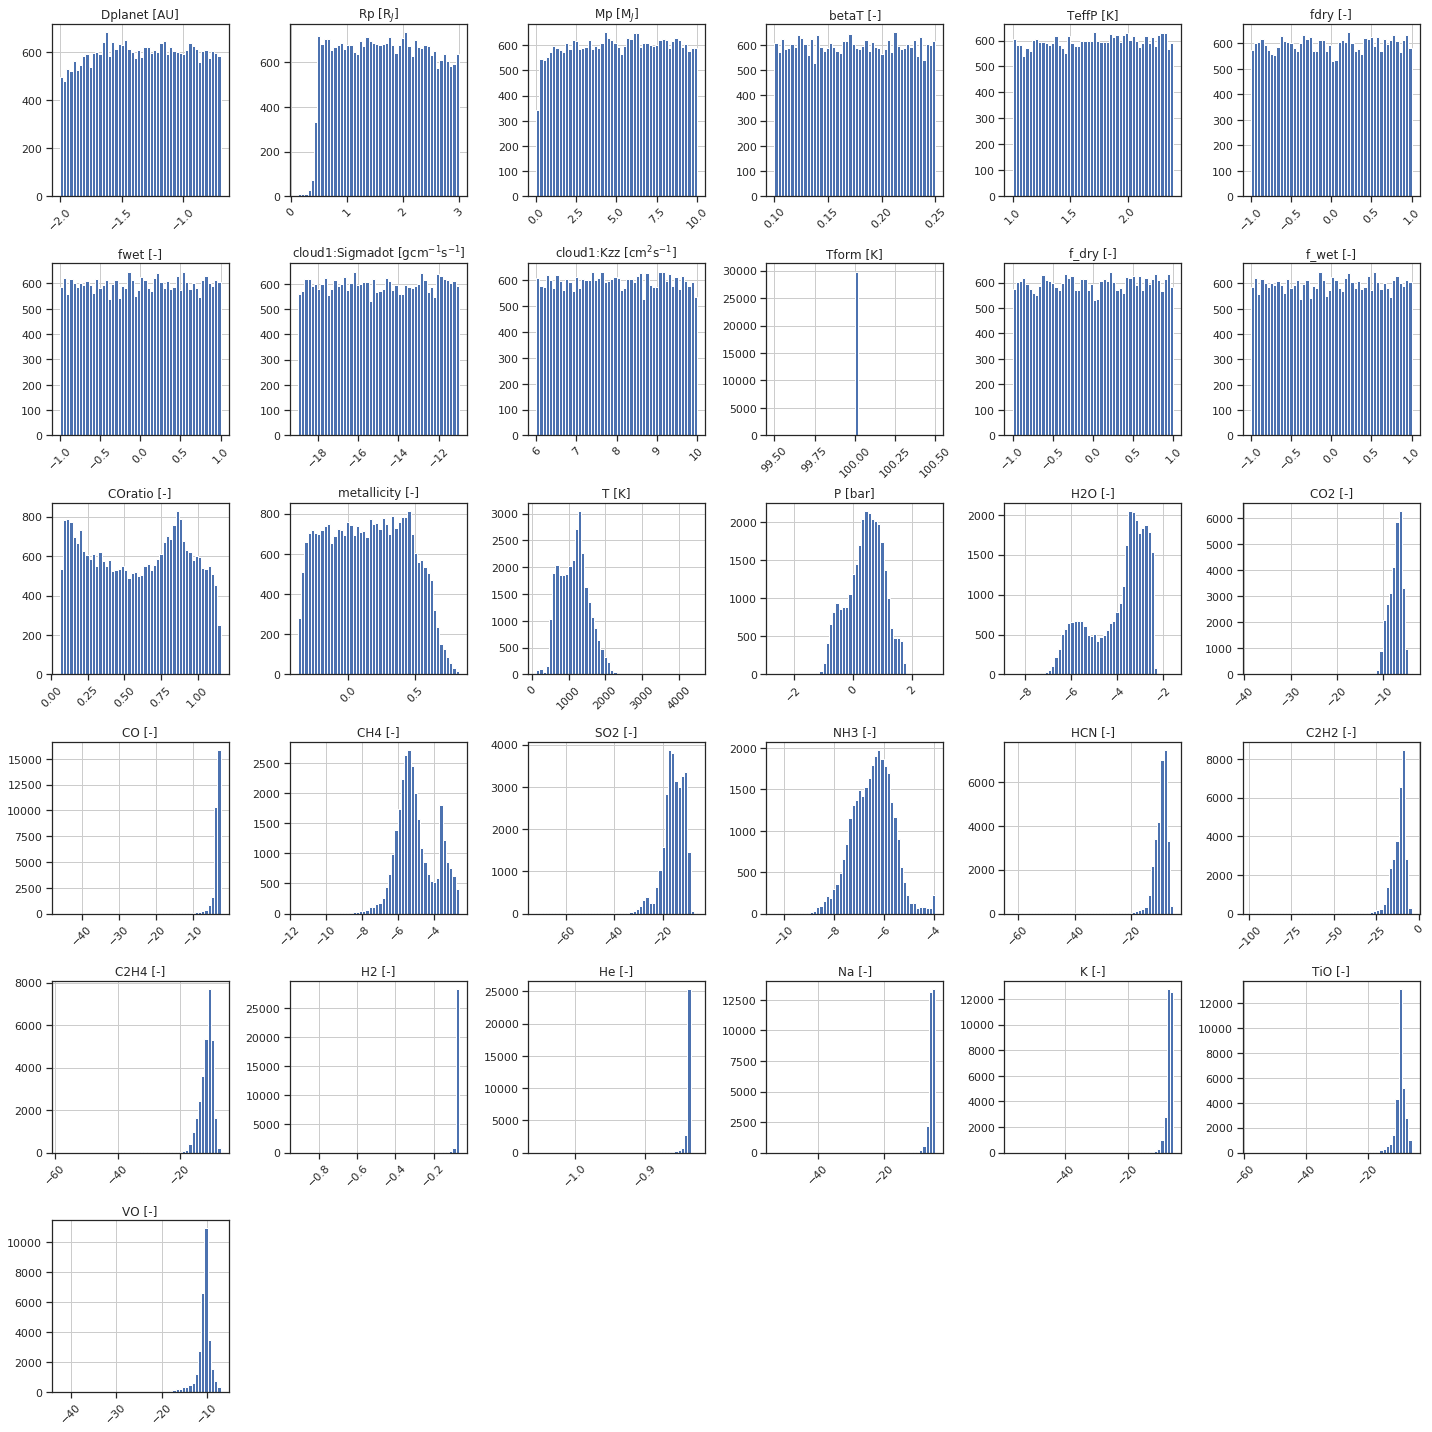
\includegraphics[scale=0.30]{figuren/complex features hist transformed.png}
    \caption{A data distribution plot containing histograms of all the complex physical features. The logarithmically sampled data has been transformed back to a logarithmic scale.}
    \label{fig:distribution}
\end{figure}




\section{Data Processing} \label{data processing}
Each spectrum with its features is encoded into an Atmospheric Spectra and Parameters Array (ASPA), as seen in Figure \ref{fig:srongan_aspa}. This essentially is a matrix containing both the spectrum, the spectrum normalisation values and the features corresponding to the spectrum. The original spectrum of 400 data points is reshaped to a shape of 25x16 to fit inside block one. The simple physical features are put into block two, one line per parameter. The same is done for the physical complex features, which are stored in block four. Block three holds the local minimum and maximum values per spectrum bin. For the simple physical models there is no data to be put inside block four, hence it is filled up with Gaussian noise according to $\mathcal{N}(0,1)$. Chapter \ref{ASPA encoding and decoding} contains a more throughout explanation of the ASPA creation.

\begin{figure} [!htb]
    \centering
    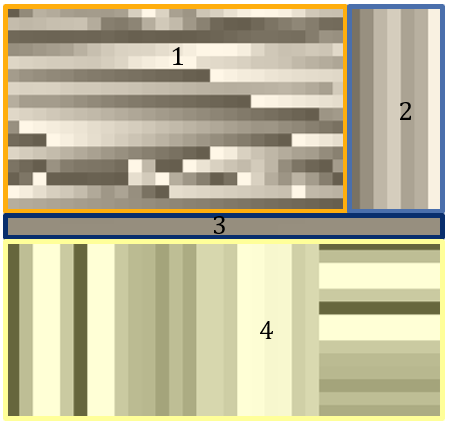
\includegraphics[scale=0.5]{figuren/srongan_aspa.png}
    \caption{The ASPA used for the complex physical models. Where block one encodes the spectrum, block 2 the simple physical parameters, block three the normalisation factors for the spectrum bins and block four the complex physical parameters.}
    \label{fig:srongan_aspa}
\end{figure}

Up to a certain extent the choice of how an ASPA is designed is completely arbitrary. The ASPA design of SRON-GAN is inspired by ExoGAN. The choice to not increase the ASPA size to 64$\times$64 has been made due to the computational power required, training instability and reasons which are given below. A noticeable difference between the ExoGAN and SRON-GAN ASPA is the size of the normalisation values and the lack of a large area for the $\mathrm{H_2O}$ abundance. 
The reasoning of \cite{zingales2018exogan} as to why these blocks take up such a large area is to put emphasis on their importance. However, the importance of the normalisation values can also be embedded into the mask used for semantic image inpainting. Giving the normalisation values e.g. a value of 10 instead of 1 within the mask used in Equation \ref{eq:inpaintingloss}.

The main reason as to why these areas have changed is as follows. The GAN is assumed to be able to completely converge and the smallest kernel sizes of 4$\times$4 pixels within the networks are taken into account. If the GAN is converged, any feature area larger than 4$\times$4 would be unnecessary. At that point the model may contain individual kernels for individual feature areas within the ASPA. Considering convolution arithmetic \cite{dumoulin2016guide}, a minimum shape of 2$\times$1 already puts an emphasis on that specific area . This is the same for the feature areas. Moreover, having blocks with a size larger than 4x4 would essentially make the network a 1D CNN. Which would be a waste of computational power.
This leads to the following situation. If the GAN has properly converged to $D(G(\boldsymbol{z}))=D(\boldsymbol{x})=0.5$ and the retrieval results of semantic image inpainting appear unreasonably inaccurate, the trivial next step would be to increase the amount of kernels within the networks. However, considering the method by which a GAN learns, having a larger area size for important physical features makes it so the GAN is likely to learn these features first. Which at the start of training has a positive influence on the results, but in the end is a waste of space within the ASPA.




\subsection{Feature Normalisation}
All information within the ASPA is linearly normalised between -1 and +1. This ensures one pixel not strongly overruling another pixel and allows for an optimal learning process. If for example one of the features lies between -10 and +10, while the rest lie between -1 and +1, the neural networks would likely be focussing on learning to predict the parameter between -10 and +10. Another downside would be the gradient being unstable for values outside of the range of -1 to +1, compared to values within this range. Due to this gradient descent might start overshooting which will essentially randomising the weights again. All normalisations are performed by the following linear transformation:
\begin{equation}
    X_{scaled}=X_{\sigma} \cdot (\mathrm{max}-\mathrm{min})+\mathrm{min}
\end{equation}
Where $\mathrm{min}=-1$, $\mathrm{max}=+1$ and
\begin{equation}
    \mathrm{X_{\sigma}} = \frac{\mathrm{X - X_{min}}}{X_{max}-X_{min}}.
\end{equation}
Where $X$ is the input value, $X_{scaled}$ is the transformed value, $X_{max}$ and $X_{min}$ are the maximum and minimum values of the variable.

\subsection{ASPA Encoding and Decoding} \label{ASPA encoding and decoding}
As mentioned in Chapter \ref{data processing}, each spectrum and its corresponding features are encoded into an ASPA. This subsection contains a conceptual example of the creation of such an ASPA. Take the following list, representing the first 9 data points of $(\frac{R_p}{R_*})^2$ with values $y=[1, 2, 3, 4, 5, 6, 7, 8, 9]$. This lists represents the values of the first 9 spectral bins of a spectrum. Each position within the list automatically corresponds to a wavelength value since each spectrum is sampled with the same spectral resolution and wavelength range. Lets also take the following example features belonging to this example spectrum: the planet radius $R_p = 10$, planet temperature $T_p = 11$ and the planet mass $M_p = 12$. This raw data now has to be processed. The features $R_p, T_p$ and $M_p$ are globally normalised between -1 and +1 by using the minimum and maximum values per parameter as received in Chapter \ref{eda}. For this example the spectrum is split up in 3 bins: $y_1=[1, 2, 3], y_2=[4, 5, 6], y_3=[7, 8, 9]$. Each bin is locally normalised between -1 and +1, e.g. the first, second and third bin minimum values would be 1, 4 and 7 respectively. After which these local minimum and maximum values are globally normalised by using the global minimum and global maximum values per bin, as received in Chapter \ref{eda}. Finally, everything is ready to be put into an ASPA:
$$ \mathrm{ASPA} = \left(\begin{matrix}1&2&3&10&11&12\\4&5&6&10&11&12\\7&8&9&10&11&12\\1&1&4&4&7&7\\3&3&6&6&9&9\end{matrix}\right) $$
For readability no normalisation has been performed in the above matrix. Notice how each value from $y$ has only one value inside the ASPA and both the features and bin normalisation values are stretched out. Decoding of the ASPA is performed using the same pipeline in reverse.




%%%%%%%%%%%%%%%%%%%%%%%%%%%%%%%%%%%%%%%%%%%%%%%%%%%%%%%%%%%%%%%%%%%%%%%%%%%%%%%%%%
\section{SRON-GAN}
Whereas ExoGAN uses a spectral range from $1 \mathrm{ \mu m}$ to $50 \mathrm{ \mu m}$, SRON-GAN uses a spectral range of $0.3 \mathrm{ \mu m}$ to $ 16 \mathrm{ \mu m}$. Both ExoGAN and SRON-GAN use a spectral resolution of $R=100$. The choice to limit SRON-GAN to a wavelength range of $(0.3-16) \mathrm{ \mu m}$ is due to little future space missions exceeding this range. The JWST is an example of a mission which goes up to $28.5 \mathrm{ \mu m}$, but measurements with this high of a wavelength highly suffer from photon noise. Making them nearly impossible to be used for retrievals, unless the measurements come from a planet orbiting an exceptionally bright host star, or if exceptionally long sampling periods are used. Notice how the normalisation factors take up less space inside the ASPA. To amplify their importance during inpainting, a non binary mask as shown in Figure \ref{fig:exogan_mask} is used. 


\begin{figure} [!htb]
    \centering
    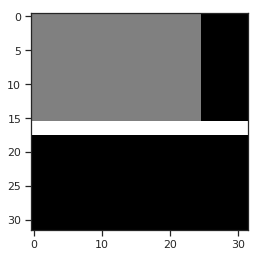
\includegraphics[scale=0.6]{figuren/exogan mask.png}
    \caption{The mask $M$ which is used for inpainting of the complex physical ASPAs. Grey represents a value of 1, white a value of 6 and black a value of 0.}
    \label{fig:exogan_mask}
\end{figure}



\subsection{Network Architecture and Hyperparameters}
When working with regular neural networks it is appropriate to perform e.g. a grid search to find the best network architecture to be used for the problem to be solved. However, the accuracy of a GAN cannot be directly verified. Combining this with the amount of computational power and time required, led to the decision to perform this task manually. To have an architecture in agreement with DCGAN, an image size of 32x32 is chosen. As for the other hyperparameters, different configurations have been tried and the one leading to the best result has been chosen. 

The network architectures of the generator and discriminator are found in Table \ref{table:srongan_architecture}. For both the simple physical models and the complex physical models the same architectures are used. The weights have been initialised by using a normal distribution of $\mathcal{N}(0,0.02)$. Gradient descent is performed by Adam \cite{kingma2014adam}. The hyperparameters for both models are found in Table \ref{table:srongan_hyperparams}. The simple physical model has been trained for 97 epochs, which took approximately 7 days using 3 NVIDIA Tesla M10 GPU's in parallel. The complex model has been trained for 2500 epochs, this took 8 days on a single NVIDIA RTX 2080 Ti GPU. Training has been stopped once the networks no longer seemed to be converging. Summarising, the general workflow is visualised in Figure \ref{fig:workflow}.

\begin{figure} [!htb]
    \centering
    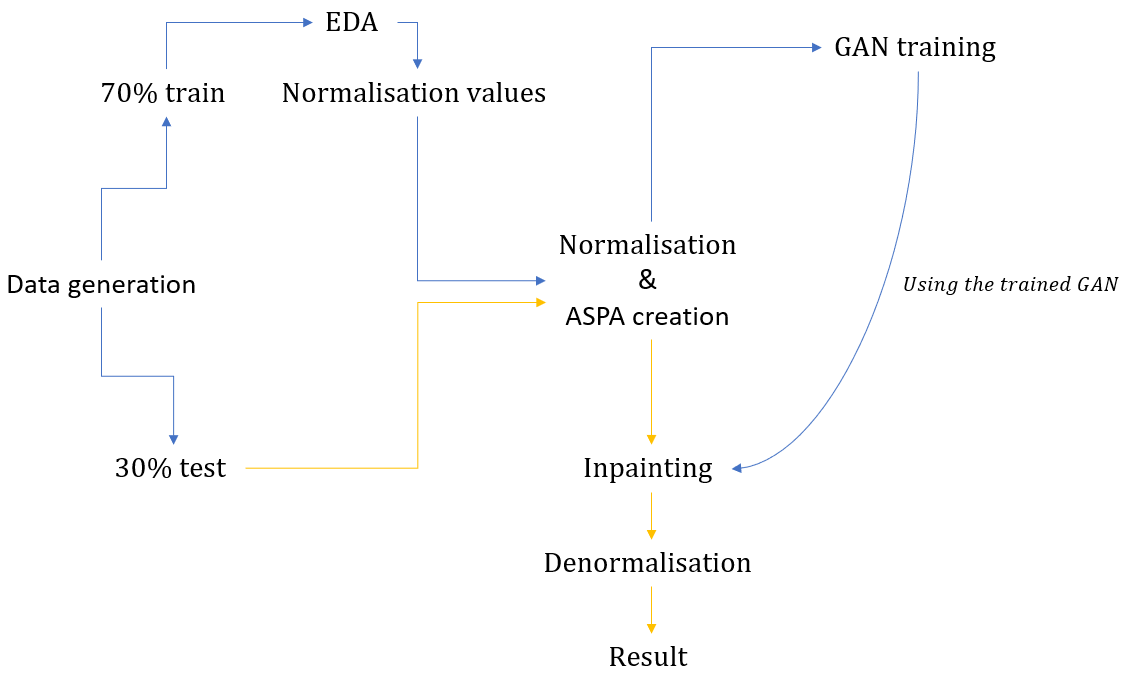
\includegraphics[scale=0.5]{figuren/wannabe_flowchart.png}
    \caption{The workflow from raw-data to SRON-GAN outputting results.}
    \label{fig:workflow}
\end{figure}








\subsection{Model Evaluation}
After choosing an architecture, four identical GANs have been trained in the same way. The best performing GAN is chosen to be used for the model evaluation. The test sets have been used to evaluate the models. The TauREX test set for the simple physical model and the ARCiS test set for the complex physical model. Semantic image inpainting is performed with the hyperparameters described in Table \ref{table:srongan_hyperparams} for both the simple and complex physical model. The inpainting of the test dataset took 3 days for the simple and complex physical model. The mean $(\mu)$ and one sigma $(1\sigma)$ percentage and absolute errors per parameter are calculated and multiple visualisations of the errors are made. Where the percentage error is given by
\begin{equation}
    \Delta y_{\%} = \frac{y-\hat{y}}{\hat{y}}\cdot 100\%
    \label{eq:perc_error}
\end{equation}
and the absolute error is given by:
\begin{equation}
    \Delta y = y-\hat{y}    
\end{equation}
With $\hat{y}$ being the ground-truth value and $y$ the retrieved value. Per performed inpainting, the contextual and perceptual loss is saved and finally visualised. These plots are used to decide whether the inpainting by Equation \ref{eq:inpaintingloss} has converged and if the contextual and perceptual loss are properly balanced. Notice how the accuracy analysis is different from the accuracy analysis performed by \cite{zingales2018exogan}. This is due to limitations in computational power, time and the fact that the accuracy analysis seems quite obscure. The complex physical model is also tested on the real data from Figure \ref{fig:nature_spectra}. This has been done by inpainting each spectrum five times and having the mean value as the prediction with the 1$\sigma$ value as the error on top of the errors as received by model evaluation. This process takes approximately 16 seconds per spectrum. The results are validated against the results from \cite{sing2016continuum} and the retrieval results of a simple retrieval performed by ARCiS, which took approximately one hour per spectrum. Considering that the radii of the host starts of the planets analysed in \citewithin{sing2016continuum}, the radii results of SRON-GAN have to be corrected for the radius of the host star. Since

\begin{equation}
    \bigg( \frac{R_p}{R_{\odot}}\bigg)^2 = F(\lambda)
\end{equation}
Where $R_p$ is the planet radius, $R_{\odot}$ the Sun radius and $F(\lambda)$ the transmission spectrum. The corrected planet radius is received by:
\begin{equation}
    R_p' = R_* \cdot R_p
\end{equation}







